% nominative
\glsaddkey
{nominative}% key
{}% default value
{\glsentrynominative}% no link cs
{\Glsentrynominative}% no link ucfirst cs
{\glsnom}% link cs
{\Glsnom}% link ucfirst cs
{\GLSnom}% link all caps cs

% genitive
\glsaddkey
{genitive}% key
{}% default value
{\glsentrygenitive}% no link cs
{\Glsentrygenitive}% no link ucfirst cs
{\glsgen}% link cs
{\Glsgen}% link ucfirst cs
{\GLSgen}% link all caps cs


% dative
\glsaddkey
{dative}% key
{}% default value
{\glsentrydative}% no link cs
{\Glsentrydative}% no link ucfirst cs
{\glsdat}% link cs
{\Glsdat}% link ucfirst cs
{\GLSdat}% link all caps cs


% accusative
\glsaddkey
{accusative}% key
{}% default value
{\glsentryaccusative}% no link cs
{\Glsentryaccusative}% no link ucfirst cs
{\glsacc}% link cs
{\Glsacc}% link ucfirst cs
{\GLSacc}% link all caps cs

% instrumental, 
\glsaddkey
{instrumental}% key
{}% default value
{\glsentryinstrumental}% no link cs
{\Glsentryinstrumental}% no link ucfirst cs
{\glsins}% link cs
{\Glsins}% link ucfirst cs
{\GLSins}% link all caps cs

% prepositional, 
\glsaddkey
{prepositional}% key
{}% default value
{\glsentryprepositional}% no link cs
{\Glsentryprepositional}% no link ucfirst cs
{\glspre}% link cs
{\Glspre}% link ucfirst cs
{\GLSpre}% link all caps cs



% glossary entries

%1 	Именительный 	Номинатив (Nominativus) 	Есть 	Кто? Что?
%2 	Родительный 	Генитив (Genitivus) 	Нет 	Кого? Чего?
%3 	Дательный 	Датив (Dativus) 	Дать 	Кому? Чему?
%4 	Винительный 	Аккузатив (Accusativus) 	Винить 	Кого? Что?
%5 	Творительный 	Аблатив (Ablativus, объединяет орудийный падеж (инструментальный, Instrumentalis) и отложительный, аблатив) 	Доволен 	Кем? Чем?
%6 	Предложный 	Препозитив (Praepositionalis) и местный (локатив, Locativus) 	Думать 	О ком? О чём? В ком? В чём? Где? (Локатив)

\newglossaryentry{cluster}
{
	name=кластер,
	description={множество объектов исходных данных, которые обладают общими признаками и выделяются этими признаками среди остальных объектов. Например, в случае кластеризации животных в один кластер могут быть выделены животные, принадлежащие одной таксономической единице (допустим, биологическому виду).}
}


\newglossaryentry{cluster-analisys}
{
	name=кластер-анализ,
	genitive = кластер-анализа,
	description={совокупность методов, разделяющих объекты таблицы наблюдений в множества (кластеры) таким образом, чтобы сходные объекты попадали в один и тот же кластер, а несходные --- в разные кластеры \cite{data-science}. Наиболее популярный метод кластер-анализа --- k-menas.}
}

\newglossaryentry{data-normalization}
{
	name=нормализация данных,
	description={преобразование данных с целью приведения всех признаков к одному масштабу и началу отчёта.}
}

\newglossaryentry{binary-cotalog}
{
	name=каталог бинарных файлов,
	description={директория файловой системы, в которой находятся исполняемые файлы программы.}
}

\newglossaryentry{text-file}
{
	name=текстовый файл,
	description={компьютерный файл, содержащий текстовые данные. Такой файл может быть отредактирован любым текстовым редактором, при этом разрешение файла не имеет значения (например, текстовым может быть файл \texttt{*.txt} или \texttt{*.csv}). }
}

\newglossaryentry{main-window}
{
	name=основное окно программы,
	description={окно Windows, которое открывается сразу после запуска программы, см. рис. \ref{fig:gui}.}
}

\newglossaryentry{main-menu}
{
	name=главное меню,
	description={элемент графического интерфейса программы, содержащий основные действия. Главное меню представляет собой строку в верхней части основного окна программы, отмечено цифрой 1 на рис. \ref{fig:gui}.}
}

\newglossaryentry{object}
{
	name=объект,
	description={сущность предметной области, соответствующая строке в таблице данных. Например, объектом может быть определённая модель смартфона, обладающая признаками: частота процессора, диагональ экрана и т.д.}
}


\newglossaryentry{feature}
{
	name=признак,
	description={числовая или категориальная характеристика объекта, соответствующая столбцу в таблице данных. Например, признаками объекта ``смартфон'' могут быть:  частота процессора, диагональ и тип экрана и т.д.}
}


\newglossaryentry{data}
{
	name=исходные данные,
	description={набор данных, представленных в виде плоской таблице и сохранённой в текстовом файле. Строка таблицы соответствует одному объекту, а столбец --- признаку. Пример таблицы исходных данных показан в разделе \ref{subsec:trainfile}.}
}

\newglossaryentry{range}
{
	name=диапазон нормирования,
	description={величина в знаменателе формулы \ref{eq:normalization}.}
}

\newglossaryentry{center}
{
	name=центр нормирования,
	description={величина вычитаемая из исходных данных в числителе формулы \ref{eq:normalization}.}
}

\newglossaryentry{Python}
{
	name=Python,
	description={язык программирования высокого уровня на котором написана программа INDACT.}
}


\newglossaryentry{util}
{
	name=утилита,
	description={вспомогательная компьютерная программа для выполнения специализированных типовых задач, связанных с работой оборудования и операционной системы. Например, для преобразования скриптов на языке Python в исполняемые \texttt{exe} файлы можно использовать утилиту \texttt{pyinstaller} (см. \url{http://www.pyinstaller.org/}).}
}

\newglossaryentry{dll}
{
	name=dll библиотека,
	description={динамически подключаемая библиотека позволяющая многократное использование различными программными приложениями (англ. \textit{Dynamic Link Library}). Примером динамически подключаемой библиотеки может служить \texttt{kernel32.dll}, реализующая основные функции MS Windows, такие как управление памятью, вводом-выводом и т.д.}
}

\newglossaryentry{console-window}
{
	name=консольное окно,
	description={окно терминала Windows. Типичный вид консольного окна показан ниже:
	\newline\begin{center}
		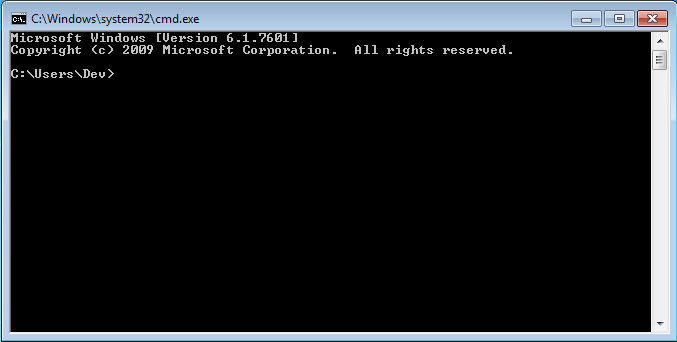
\includegraphics[width=0.75\textwidth]{img/terminalexample}
	\end{center}}
}

\newglossaryentry{scatter-plot}
{
	name=scatter plot,
	description={способ графического отображения двумерных данных на плоскости при котором каждый объект соответствует точке с координатами, равными значениям признаков этого объекта.}
}

\newglossaryentry{marker}
{
	name=метка,
	description={вспомогательный символ, присваиваемый пользователем для  определённого признака. Метки используются для выбора роли признака при построении диаграмм (например, scatter plot). Предусмотрено 3 вида меток: ``\texttt{X}'', ``\texttt{Y}'', ``\texttt{C}''. Первый вид означает что отмеченный признак будет соответствовать координатам объекта по оси абсцисс, второй --- по оси ординат, а третий, что цвет (\textit{Color}) точки будет выбираться в соответствии со значением отмеченного признака.}
}

\newglossaryentry{statusbar}
{
	name=строка состояния,
	description={элемент графического интерфейса, расположенный в нижней части основного окна программы, предназначенный для вывода текстовой информации вспомогательного характера
	\newline\begin{center}
		
\includegraphics[width=0.75\textwidth]{img2/statusbar.png}
	\end{center}}
}

% acronim entries
\newacronym{OS}{ОС}{Операционная Система}
\newacronym{OZU}{ОЗУ}{Оперативное Запоминающее Устройство}
\newacronym{PC}{ПК}{Персональный Компьютер}
\newacronym{PO}{ПО}{Программное Обеспечение}
\newacronym{LKM}{ЛКМ}{Левая Кнопка Мыши}
\newacronym{PKM}{ПКМ}{Правая Кнопка Мыши}
\newacronym{SVD}{SVD}{Singular Value Decomposition}
\newacronym{INDACT}{INDACT}{Система Интеллектуальной Кластеризации (INtelligent DAta Clustering Toolkit)}